\title{Absorption and Fluorescence in Ruby Crystal}

\newcommand{\abstractText}{\noindent
The unique optical properties of the ruby crystal that make it effective as a lasing medium were measured using a simple optical setup. Ruby’s absorption of visible light was shown to be strongest at 420 and 550 nm, corresponding to its physical appearance as transparent pink. While the ruby crystal was illuminated with a 532 nm green laser, the R-line fluorescence peaked at 693.5 $\pm$ 1.1 nm. Finally, the fluorescence lifetime of ruby was measured by pulsing the laser with a signal generator and capturing the decaying fluorescence on a digital oscilloscope using a  photodiode. An exponential decay time-constant of 3.6 $\pm$ 0.1 ms was obtained, corresponding to the fluorescence lifetime. 
}

%%%%%%%%%%%%%%%%%
% Configuration %
%%%%%%%%%%%%%%%%%

\documentclass[11pt, a4paper, twocolumn]{article}

%% Authors and affiliations
\usepackage{authblk}
\author[1]{William Cutler}
\author[1]{Jack Donaghue}
\author[1]{Haridas Kumarakuru}
\author[1]{Don Heiman}
\affil[1]{\footnotesize{\textit{Department of Physics, Northeastern University, Boston, MA 02115, USA}}}

\usepackage{xurl}
\usepackage[comma, sort&compress]{natbib}
\usepackage{abstract}
\usepackage[separate-uncertainty=true]{siunitx}
\usepackage{graphicx}
\renewcommand{\abstractnamefont}{\normalfont\bfseries}
\renewcommand{\abstracttextfont}{\normalfont\small\itshape}
\usepackage{lipsum}

% Any configuration that should be done before the end of the preamble:
\usepackage{hyperref}
\usepackage{float}
\usepackage{flushend}
\hypersetup{colorlinks=true, urlcolor=blue, linkcolor=blue, citecolor=blue}
\usepackage[a4paper, total={7in, 10in}]{geometry}
\setlength{\columnsep}{24pt}
\begin{document}
%%%%%%%%%%%%
% Abstract %
%%%%%%%%%%%%

\twocolumn[
  \begin{@twocolumnfalse}
    \maketitle
    \begin{abstract}
      \abstractText
      \newline
      \newline
    \end{abstract}
  \end{@twocolumnfalse}
]

%%%%%%%%%%%
% Article %
%%%%%%%%%%%
\pretolerance=5000

\section*{Introduction}
The absorption and fluorescence emission spectra have long been used to identify, characterize, and study materials \cite{BrittanicaSpectroscopy}. In lasing mediums, these properties govern the excitation and emission spectra of the laser, respectively. Ruby, which was used as the lasing medium in the first working laser, is composed of a small concentration of Cr ions doped in a crystalline sapphire ($Al_2O_3$) matrix. Studies of ruby absorption typically use a spectrophotometer and measure two broad absorption peaks centered near \SI{410}{\nm} and \SI{550}{\nm} \cite{Esposti,Kusuma,Song}. Song et. al. also calculate an absorption coefficient for these wavelengths according to Beer-Lambert's law \cite{Song}. Spectrometers with high resolution additionally detect a small doublet absorption peak near \SI{694}{\nm}.

The fluorescence spectrum of ruby at room temperature has been reported throughout the early 1900's with a double peak at \SI{692.7}{\nm} and \SI{694.2}{\nm}, corresponding to the characteristic $R_1$ and $R_2$ lines \cite{Kumari, Mani}. With lower resolution instruments, only a single primary peak was detected at \SI{694.2}{\nm} \cite{Esposti}. Other fluorescence lines have been detected near these peaks at 671, 688, 695, and \SI{710}{\nm} \cite{Kusuma}, corresponding to fluorescence mechanisms other than the primary R-line, such as exchange-coupled Cr ion pairs (N - lines) \cite{Yamaoka}.

The effectiveness of ruby as a lasing medium is derived from its ability to maintain a population inversion between the ground state and the metastable state, shown as 'Level 2' in Figure \ref{fig:Population-inversion-3level}. The stability of this metastable state can be measured by the fluorescence lifetime, which relates to how long the crystal will fluoresce in the absence of pumping, and therefore the time for which there is a sizeable metastable population. Whereas most materials have nano or picosecond fluorescence lifetimes \cite{Berezin}, ruby’s fluorescence lasts milliseconds, long enough to hold a population inversion for a working laser.

\begin{figure}
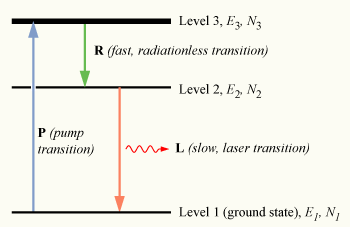
\includegraphics[width=\linewidth]{Population-inversion-3level.png}
\caption{\textit{Sample energy level diagram showing three phases of fluorescence: pumping, nonradiative relaxation, and fluorescent relaxation.}}
\label{fig:Population-inversion-3level}
\end{figure}

A fluorescence lifetime of around \SI{3.5}{\ms} is typically reported, but this measurement is dependent on a number of factors. Investigations of the temperature dependence show that lifetime decreases for temperatures above room temperature \cite{Seat, Nelson}. Fluorescence lifetime was shown to increase with the diameter of the ruby sample as emitted photons are reabsorbed more frequently in larger samples \cite{Jones}. The doping concentration can also affect the lifetime \cite{Brown}. Brown found that at room temperature, doping concentrations between 0.005\% and 0.1\% yielded lifetimes in the range of 3-\SI{4}{\ms}.

Many investigations use a single exponential fit to obtain the fluorescence lifetime, but others use a double exponential fit based on theoretical knowledge and the shape of the residuals for single exponential fits \cite{McBane, Jones}. 

\section*{Experimental Setup}

The apparatus and procedure for this investigation is based on \cite{Heiman}. A diagram of the optical setup is shown in Figure \ref{fig:laserBenchDiagram}, and the ruby crystal itself in Figure \ref{fig:rubyPhoto}. The ruby sample used was approximately 0.05\% Cr. For absorption measurements, white light from a Maglite was sent onto the crystal, and the transmitted light was captured by a fiber optic, which was then sent to the spectrometer, an OceanOptics USB 2000 \cite{SpectrometerData}. The ruby mount was not fixed to the table, so that it could be moved out of the path of the white light in order to capture the unabsorbed light. A black cloth ensured no interference from background room light. Note that the flashlight must have a wide-spectrum incandescent bulb rather than a narrow-band LED.

\begin{figure}
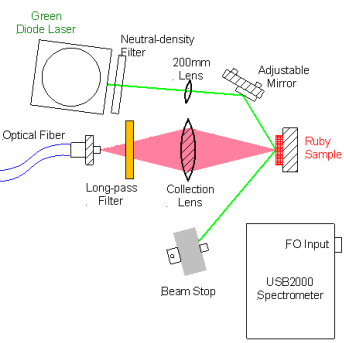
\includegraphics[width=\linewidth]{laserBenchDiagram.png}
\caption{\textit{Diagram of fluorescence spectrum measurement setup showing the laser beam in green and R-line fluorescence in red \cite{Heiman}.}}
\label{fig:laserBenchDiagram}
\end{figure}

\begin{figure} %[]
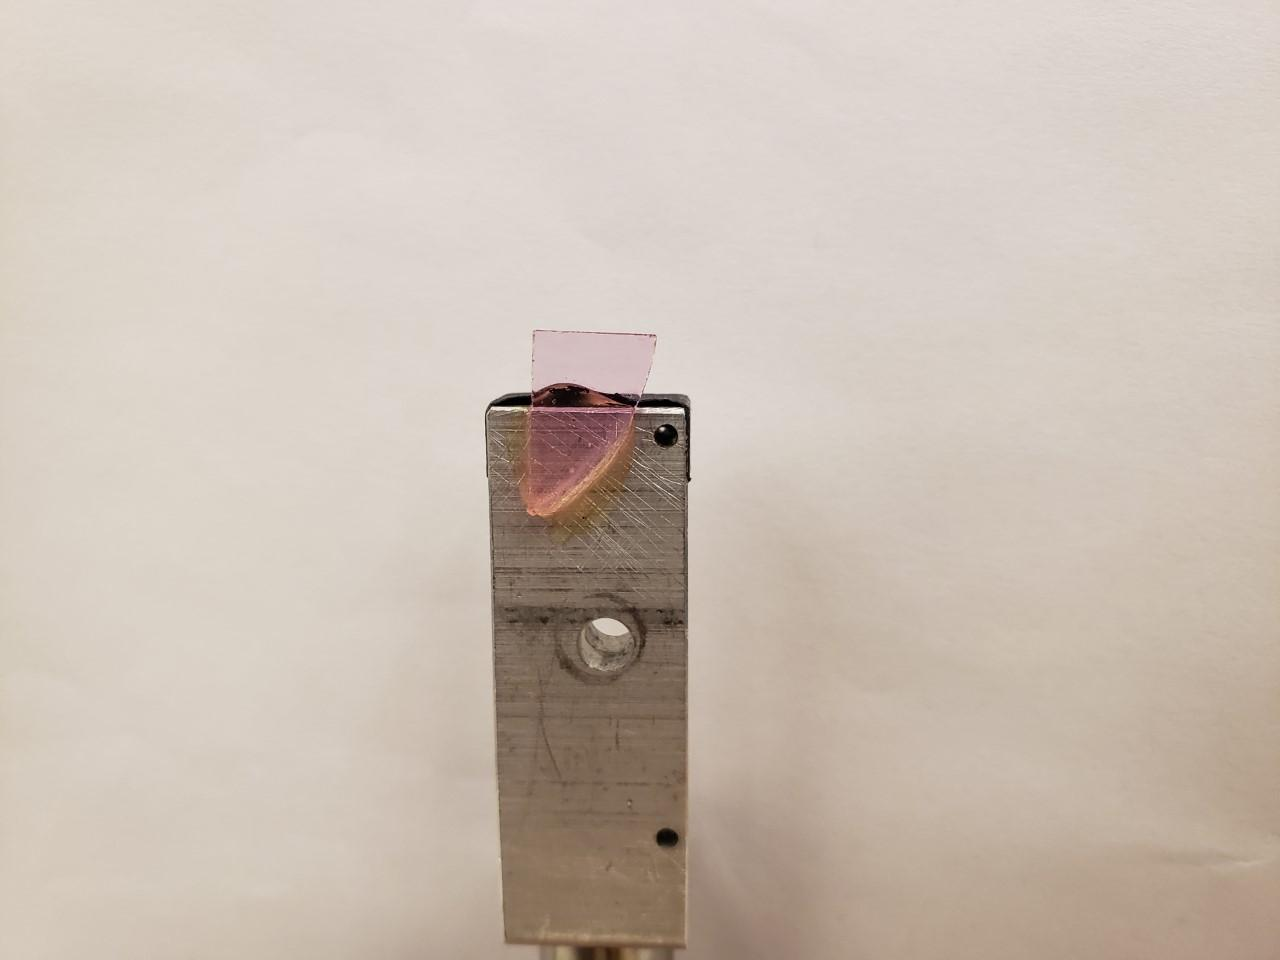
\includegraphics[width=\linewidth]{rubyPhoto.png}
\caption{\textit{Photograph of the transparent pink ruby crystal used throughout this study. The laser and white light were directed to the top part of the crystal, above the metal stand.}}
\label{fig:rubyPhoto}
\end{figure}

For fluorescence measurement, initial alignment began by positioning the fiber optic mount and focusing lens. A white light was placed at the end of the fiber optic such that its light would pass through the fiber, become focused by the lens, and appear on the ruby sample. Adjustments to the mount and collection lens were made until this light was maximally focused on the ruby, since that would ensure that the fluoresced light would be focused on the fiber optic for transmission to the spectrometer. Additionally, the laser was briefly turned on during this adjustment to observe that the white light and laser both struck the ruby at the same location. These steps ensured that the fluoresced light that reached the fiber optic was maximized at the spectrometer.

\section*{Results}
\subsection*{Transmission and Absorption}

The transmittance of a material, $T$, is simply the fraction of incident light power (or intensity) that passes through the material:
\setlength{\abovedisplayskip}{8pt}
\setlength{\belowdisplayskip}{8pt}

\begin{equation}\label{eq1}
    T=I/I_0. 
\end{equation}

$I$ represents the transmitted intensity and $I_0$ is the incident intensity measured from the unobstructed Maglite. Figure \ref{fig:doubleIntensityMeasurement} shows the spectra of $I$ and $I_0$. Note that there is a larger difference in intensity in the 500-600 nm region, indicating a minimum in the transmission spectrum corresponding to an absorption peak. These extrema can be observed in Figures \ref{fig:transmissionSpectrum} and \ref{fig:absorptionSpectrumFocused},  respectively.

\begin{figure} %[]
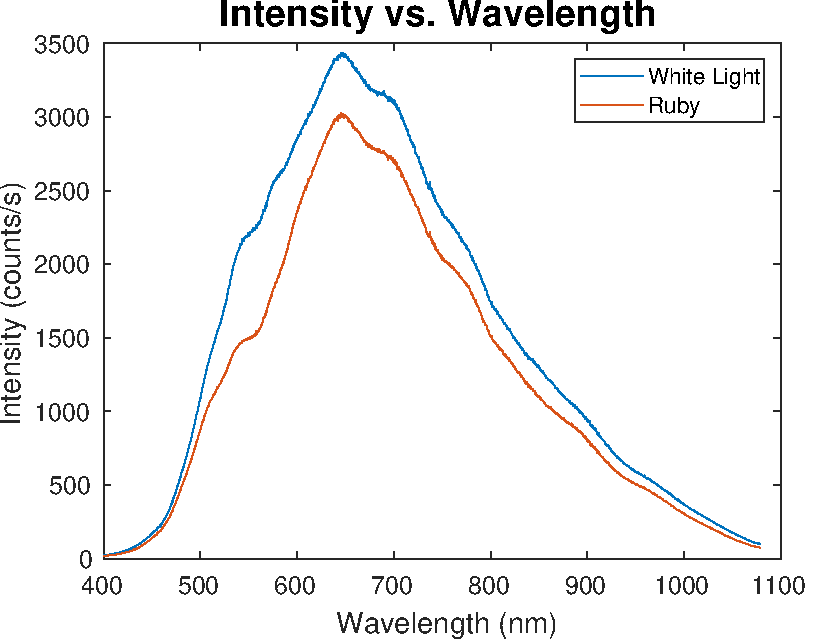
\includegraphics[width=\linewidth]{doubleIntensityMeasurement.pdf}
\caption{\textit{Spectrum of intensities for bare white light (blue line), and transmitted white light (orange line) after passing through ruby.}}
\label{fig:doubleIntensityMeasurement}
\end{figure}

\begin{figure} %[H]
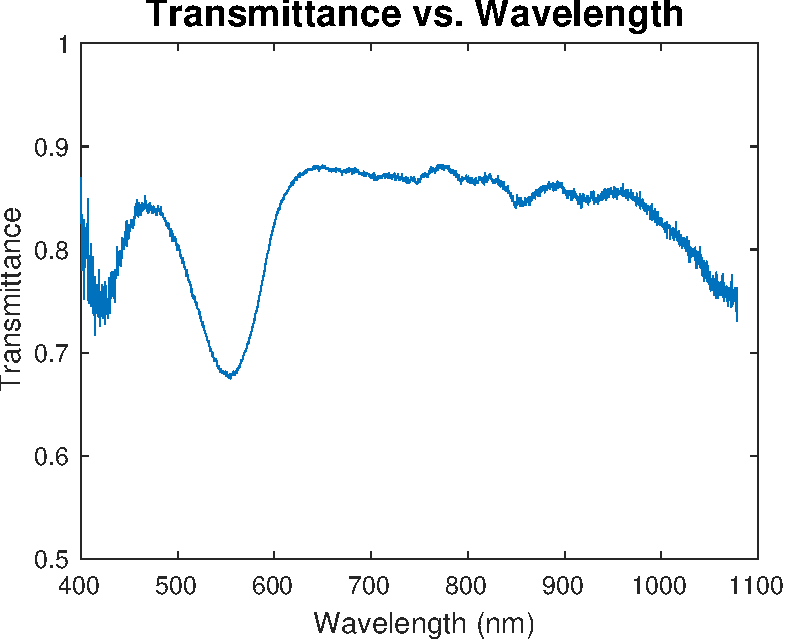
\includegraphics[width=\linewidth]{transmissionSpectrum.pdf}
\caption{\textit{Transmission spectrum of the ruby crystal showing prominent minima at 420 nm and 550 nm.}}
\label{fig:transmissionSpectrum}
\end{figure}

In order to convert the transmission spectrum into an absorption spectrum, the reflection losses from the surfaces must be taken into account. The reflectivity of the ruby is given by the formula below, and represents the proportion of incident light reflected at one ruby-air interface:

\begin{equation} \label{eq2}
    R=\frac{(n-1)^2}{(n+1)^2},
\end{equation}

where $n$ is the refractive index of ruby. 

The absorption coefficient, $\alpha$, which governs the rate of the exponential decay of light intensity as it travels along the length of the material, was calculated using Equation \ref{eq3} as derived from Beer-Lambert's law \cite{BeerLambert}.

\begin{equation}\label{eq3}
   \alpha = \frac{1}{L}\ln(\frac{I_0}{I}(1-R)^2),
\end{equation}

$L$ is the length of the ruby measured along the path of the light passing through it (thickness). Below are the relevant quantities used for calculating the absorption coefficient:
\\\\
\begin{tabular}{ll}
\textbf{Index of Refraction} & 1.76 ± 0.02 \cite{rubyRefraction}    \\
\textbf{Reflectivity}        & 7.58 ± 0.11\%  \\
\textbf{Length}              & 2.00 ± 0.05 mm  
\end{tabular}
\\
% \begin{figure}[H]
% 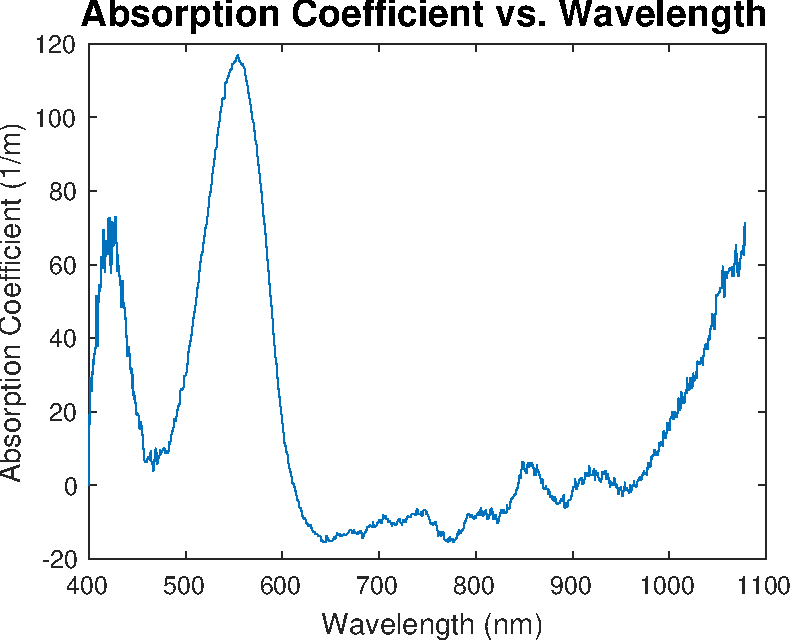
\includegraphics[width=\linewidth]{absorptionSpectrum.pdf}
% \caption{Absorption spectrum of the ruby crystal with two absorption peaks centered at 410 nm and 550 nm}
% \label{fig:intensities}
% \end{figure}

\begin{figure}[]
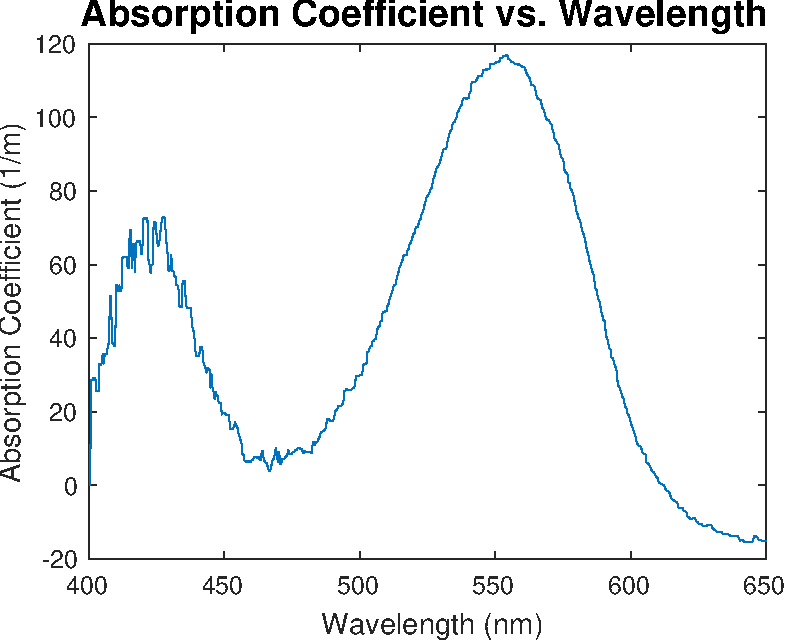
\includegraphics[width=\linewidth]{absorptionSpectrumFocused.pdf}
\caption{\textit{Absorption spectrum of the ruby crystal showing two broad absorption peaks centered at 410 nm and 550 nm.}}
\label{fig:absorptionSpectrumFocused}
\end{figure}

% \begin{figure}[]
% 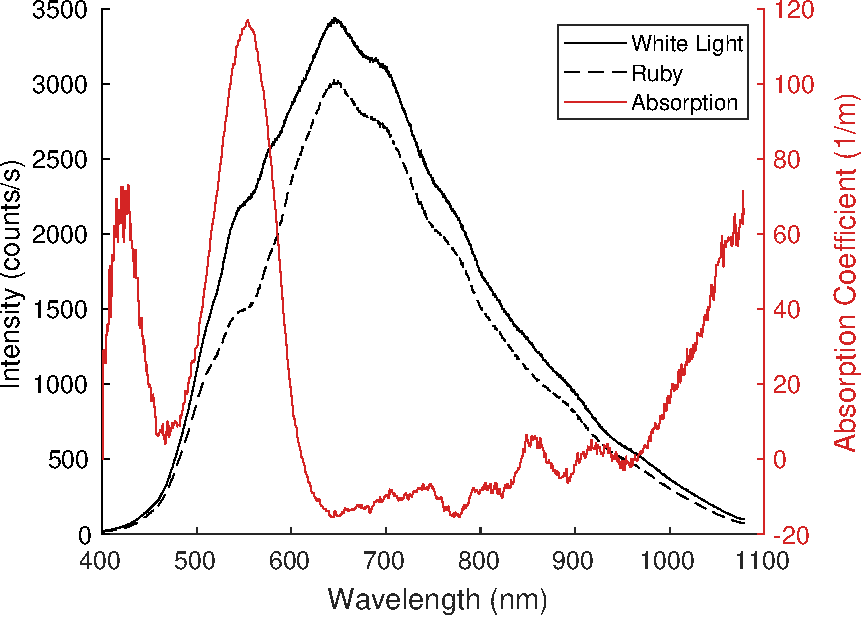
\includegraphics[width=\linewidth]{absorptionAndIntensitySpectra.pdf}
% \caption{\textit{Combination of intensity and absorption spectra showing a correspondence between the strongest absorption peak and intensity differential between measurements with and without ruby.}

% \label{fig:intensities}
% \end{figure}

Because transmittance was recorded as a function of wavelength and other quantities are constant, the absorption coefficient is also a function of wavelength, yielding the absorption spectrum shown in Figure \ref{fig:absorptionSpectrumFocused}. The absorption has broad peaks at 420 ± 5 nm and 553 ± 1 nm wavelengths, corresponding to absorption coefficients of 66.5 ± 0.9 m$^{-1}$ and 116.7 ± 1.1 m$^{-1}$, respectively. 

With these values, the intensity of the light would be expected decrease by a factor of $e$ after traversing 15 ± 2 mm and 8.57 ± 0.08 mm, respectively. That these lengths are much greater than the actual thickness of the ruby crystal is consistent with the fact that it is mostly transparent. Furthermore, the pink color of the crystal is due to these broad absorption bands of Cr$^{3+}$ in the violet (400 - 450 nm) and yellow-green (500 - 600 nm) regions, with a minimum of absorption in the deep red region ($>$ 650 nm).

\subsection*{Fluorescence Spectrum}

Peak R-line fluorescence occurred at 693.5 nm, the deep red color emitted by a ruby laser, with an 8 nm full-width at half-maximun (FWHM) linewidth for the entire peak, shown in Figure \ref{fig:fluorescenceSpectrum}. A streak of red light could be seen by looking down into the top of the ruby crystal. Because the spectrometer used had a resolution of $>$1 nm, it was unable to discern the double peak found in other experiments, instead showing a single peak spanning the entire double peak range (692.7 to 694.3 nm). Also captured by the spectrometer were smaller peaks on either side of the primary R-line, at 670 nm and 710 nm, corresponding to neighbor (N) lines and side bands, respectively, as detected by Kusuma \cite{Kusuma}.

\begin{figure} [t]
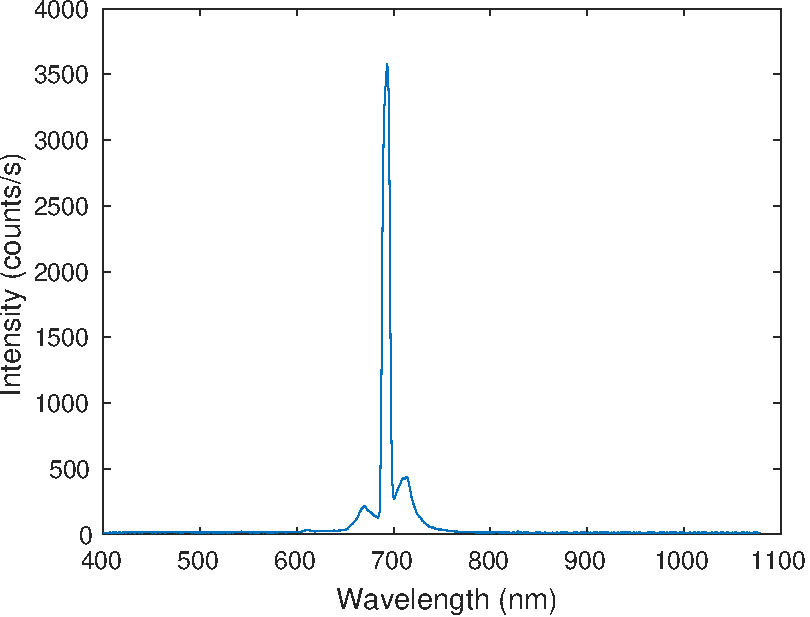
\includegraphics[width=\linewidth]{fluorescenceSpectrum.pdf}
\caption{\textit{Fluorescence spectrum of the ruby crystal showing fluorescence near the R-line peak at 693.5 nm.}}
\label{fig:fluorescenceSpectrum}
\end{figure}

\subsection*{Fluorescence Lifetime}
Important aspects of the fluorescence process were observed by measuring the strength of fluorescence across time for a ruby crystal subjected to a pulsed laser. The diagram in Figure \ref{fig:decayMeasurementSchematic} illustrates the setup and signal paths. The laser was pulsed by a 10-Hz square-wave function generator and the ruby fluorescence was captured by a photo-diode. Meanwhile, the two-channel oscilloscope simultaneously recorded the square wave that pulsed the laser (orange arrow) and the fluorescence signal captured by the photodiode (blue arrow). A photograph of the optical bench for this process is shown in Figure \ref{fig:laserBenchPhoto}.

\begin{figure}[H]
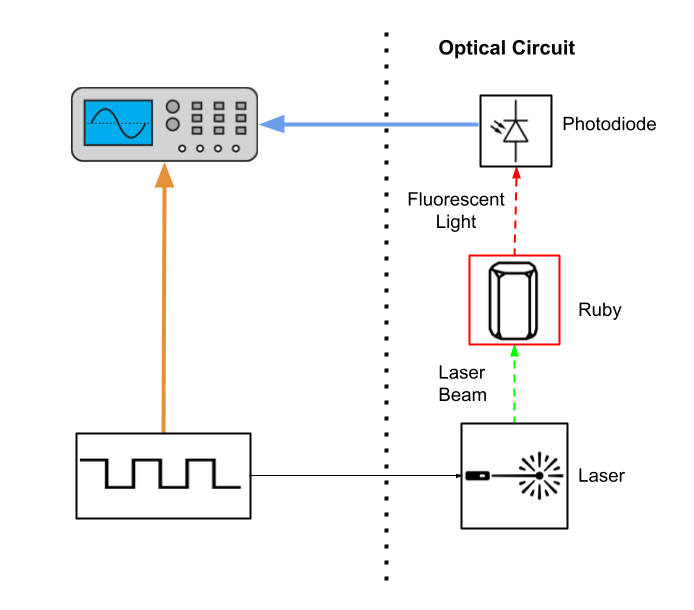
\includegraphics[width=\linewidth]{decayMeasurementSchematic.png}
\caption{\textit{Schematic illustration of fluorescence lifetime measurement showing the square-wave electrical signal of the laser and fluorescence input to the oscilloscope.}}
\label{fig:decayMeasurementSchematic}
\end{figure}

\begin{figure} %[]
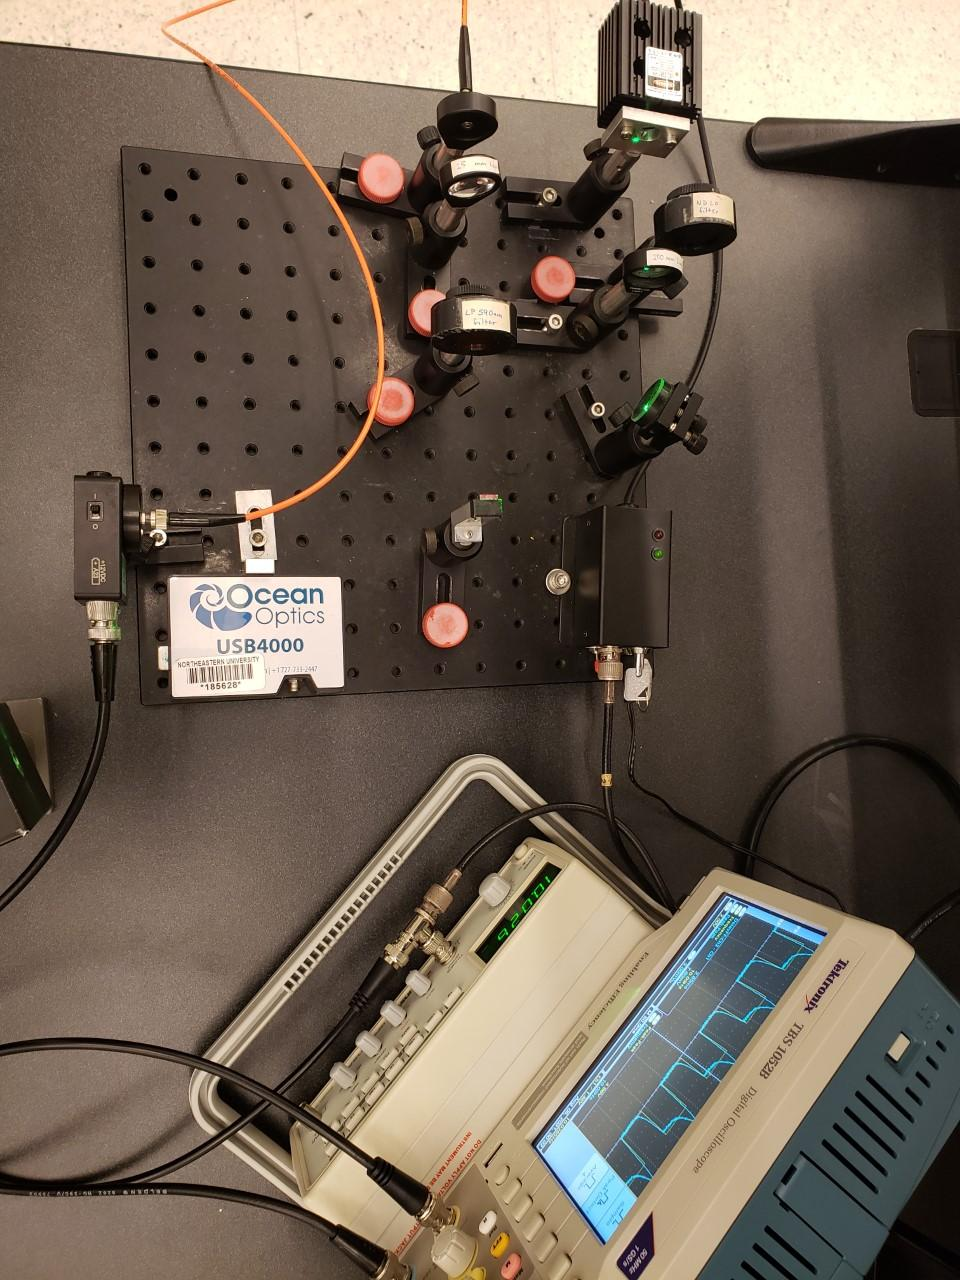
\includegraphics[width=\linewidth, height=\linewidth]{laserBenchPhoto.png}
\caption{\textit{Photograph of laser bench setup for measuring fluorescence lifetime.
}}
\label{fig:laserBenchPhoto}
\end{figure}

One period of the 10-Hz signal captured by the oscilloscope is shown in Figure \ref{fig:fluorescencePeriod}, with the square wave in blue and the fluorescence in orange. It shows a series of distinct phases outlining the entire process of fluorescence. Initially, the fluorescence rises sharply from t = 0.015 to 0.025 s, as excited Cr ions fluoresce back to the ground state. From t = 0.025 s until the laser pulse turns off at \SI{0.05}{\s}, the fluorescence is in saturation, as the rate of emission reaches the rate of excitation. Finally, after \SI{0.05}{\s}, with the laser turned off, fluorescence continues, but its rate decreases exponentially. The rate of this exponential decay is governed by the probability that a given metastable Cr ion will fluoresce and relax in a given period of time. 

\begin{figure} %[]
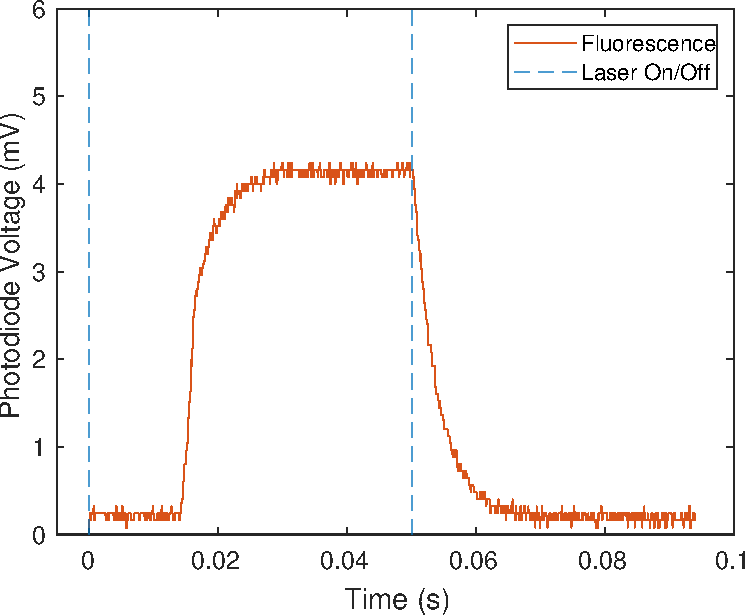
\includegraphics[width=\linewidth]{fluorescencePeriod.pdf}
\caption{\textit{Oscilloscope traces for one period of laser pulse at 10 Hz, showing the fluorescence emission in orange and the laser excitation in blue that ends at 0.05 s.}}
\label{fig:fluorescencePeriod}
\end{figure}

The fluorescence decay was isolated from the oscilloscope data, and a single exponential fit of the form $y = ae^{-x/\tau} + c$ was applied to determine the fluorescence lifetime $\tau$ = 3.6 ± 0.1 ms, as shown in Figure \ref{fig:decayFit}. The inclusion of a constant in the fit was important because the photodiode voltage does not decay to 0, but has a small background value below 0.5 mV.

\begin{figure} %[]
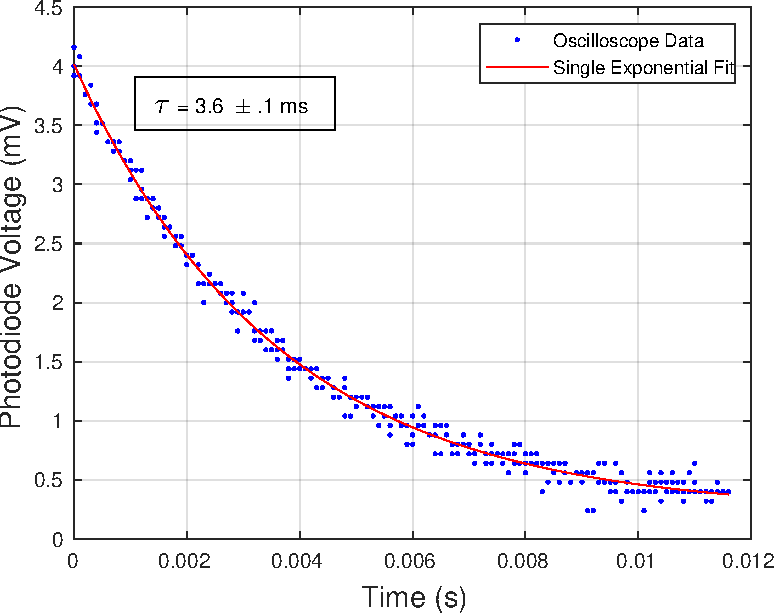
\includegraphics[width=\linewidth]{decayFit.pdf}
\caption{\textit{R-line fluorescence data as a function of time in blue points. The red curve is a MATLAB fit to the data.}
}
\label{fig:decayFit}
\end{figure}

A single exponential fit is reported here for its simplicity and interpretability. Furthermore, it provided a high correlation ($R^2=0.993$), and its residual plot, shown in Figure \ref{fig:decayResiduals}, has no discernible pattern, unlike those reported by \cite{Jones} in justification of the double exponential. This is not to deny the theoretical relevance of a double exponential in describing the fluorescence process, but rather to demonstrate that the single exponential fits the data remarkably well, beyond mere visual inspection.

\begin{figure} %[]
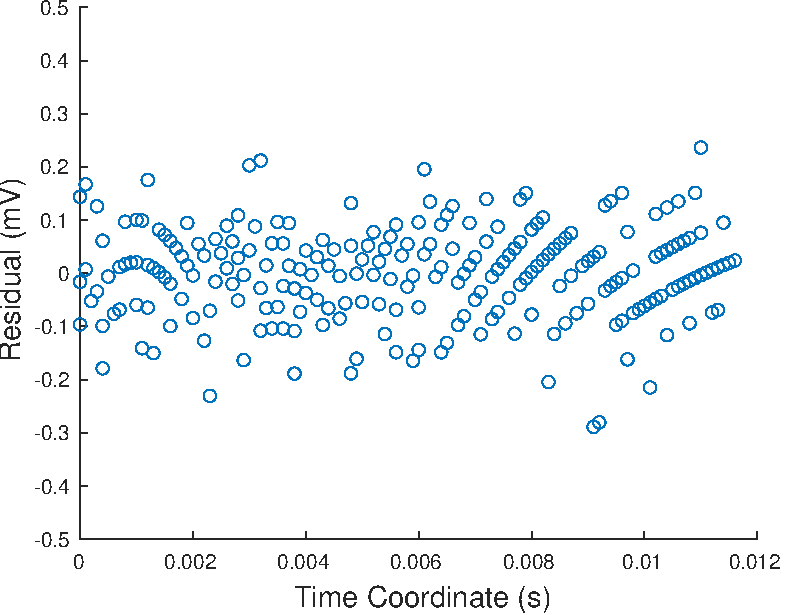
\includegraphics[width=\linewidth]{decayResiduals.pdf}
\caption{\textit{Residual plot for the single exponential fit to the ruby fluorescence data in the previous figure, showing no discernible pattern that might indicate a more complex fit is needed.}}
\label{fig:decayResiduals}
\end{figure}
\newpage
The time constant represents the amount of time needed for the fluorescence emission to decrease to $1/e$ of its original value. Whereas many materials exhibit fluorescence lifetimes on the order of nanoseconds or picoseconds, ruby’s fluorescence lasts multiple milliseconds, a significant factor in its effectiveness as a lasing medium.

\section*{Discussion}
The experiments and analysis performed concern the optical properties of the ruby crystal sample. Peak absorption was observed at wavelengths of 420 ± 5 nm and 553 ± 1 nm with absorption lengths of 15 ± 2 mm and 8.57 ± 0.08 mm, respectively. 

The transmission and absorption spectra of the ruby were consistent with its visual appearance as a transparent pink crystal. The noise in the 420 nm absorption peak (and transmission valley) is due to the low overall intensity of the Maglite seen in Figure \ref{fig:doubleIntensityMeasurement}. Therefore, a light with more intensity in this region would yield a less noisy transmission and absorption spectrum.

The fluorescence showed a singular clear peak at 693.5 ± 1.1 nm. This range would encompass the double line of the ruby fluorescence spectrum at 692 and 694 nm recorded by \cite{Kumari, Mani}. Using a single exponential fit, the R-line fluorescence lifetime was found to be 3.6 ± 0.1 ms.

\subsection*{Acknowledgements}
We would like to thank Nathaniel Avish and Hongwei Chen for their help in the laboratory as teaching assistants for the Advanced Physics Laboratory section for which this experiment was introduced. We would also like to thank the Northeastern University Department of Physics for financially supporting our experience at the ASEE-NE 2021 conference.
%%%%%%%%%%%%%%
% References %
%%%%%%%%%%%%%%
\nocite{*}
\bibliographystyle{unsrt}
\footnotesize{\bibliography{reference}}
\end{document}

